\chapter{Vorstellung der SmartFactory@EH-Anlage}\label{ch:experiments}

Die \textbf{SmartFactory-Anlage} ist eine speziell für Schulungszwecke konzipierte Automatisierungsanlage, die von der Abteilung 
\textbf{Expert House} der Siemens AG entwickelt wurde. Sie dient als Trainingsplattform für Auszubildende, Studierende und Mitarbeitern, um praxisnahe 
Erfahrungen in der Automatisierungstechnik zu sammeln und mit einer Vielzahl von Produkten aus dem Siemens-Katalog vertraut zu werden. Die 
Anlage simuliert eine Flaschenabfüllung und wird zur Ausbildung sowie zum Testen von neuen Technologien und Funktionen genutzt.

Die Anlage kann über drei Modulbetriebsarten gesteuert werden: \textbf{Einrichtungsbetrieb}, \textbf{Handbetrieb} und \textbf{Automatikbetrieb}, 
sowie zwei Anlagenbetriebsarten: \textbf{Modularbetrieb} und \textbf{Inselbetrieb}. Im \textbf{Einrichtungsbetrieb} kann der Bediener alle Anlagenteile 
uneingeschränkt bewegen, auch wenn dies zu Beschädigungen führen könnte. Der \textbf{Handbetrieb} ermöglicht es, einzelne Funktionen 
auszuführen, wie das Befüllen einer Flasche oder das Entleeren eines Bandes. Im \textbf{Automatikbetrieb} läuft die Anlage vollständig 
automatisiert und erfordert nur im Fehlerfall, zum Anlegen eines Auftrags oder bei einer Bedieneranforderung, einen Bediener. Eine Bedieneranforderung
wäre hier zum Beispiel das manuelle Entleeren der Kommissionierbahn oder das Entleeren eines Deckelausschussbands. Während es im \textbf{Modularbetrieb}
darum geht, dass die Anlage als Ganzes betrachtet wird, also eine Kommunikation mit Nachbarstationen aufgenommen werden kann,
 wird im \textbf{Inselbetrieb} jedes Modul einzeln betrachtet und getestet.

Der modulare Aufbau der Anlage umfasst sieben verschiedene Teilmodule: die \textbf{Abfüllstation}, die \textbf{Qualitätskontrolle}, die 
\textbf{Kommissionierbahn}, die \textbf{Eckstation}, die \textbf{Recyclingstation}, den \textbf{Delta-Picker} und das \textbf{MPS-Modul}. 
Diese Stationen sind durch ein Kreislaufsystem miteinander verbunden, wobei die Flaschen von der Abfüllstation über die verschiedenen 
Stationen transportiert werden. Im Kreislaufsystem werden die Flaschen am Ende des Prozesses, nach dem Recycling, wieder zur erneuten 
Verarbeitung bereitgestellt.

Jedes Modul der Anlage hat einen spezifischen Schwerpunkt und ist mit ähnlicher Hardware ausgestattet, einschließlich einer 
\textbf{Siemens-Simatic S7-1500 Speicherprogrammierbaren Steuerung} (SPS), außer dem Quality-Gate, bei dem ältere Steuerungstechnik 
mit einer ET200Sp verbaut ist, einem \textbf{Siemens HMI} (Human-Machine Interface) für 
Statusmeldungen und Benutzereingaben sowie Transportbändern. Zudem sind an einigen Stationen pneumatisch betriebene Greifer und 
RFID-Schreib-Lesegeräte verbaut, die eine präzise Steuerung und Überwachung der Anlage ermöglichen. Die Anlage läuft iterativ, was 
bedeutet, dass nach Abschluss des Kreislaufs die Flaschen, Deckel und Kugeln für die erneute Abfüllung bereitgestellt werden.

Die Funktionsweise der einzelnen Stationen im \textbf{Automatikbetrieb} ist wie folgt: In der \textbf{Abfüllstation} werden die Flaschen mit 
Kugeln befüllt, bevor sie in die nächsten Stationen weitergeleitet werden. In der \textbf{Qualitätskontrolle} wird die Qualität der befüllten 
Flaschen geprüft. Danach erfolgt in der \textbf{Kommissionierbahn} und der \textbf{Eckstation} die Sortierung der Flaschen sowie eine weitere 
Qualitätsprüfung. Der Kreislauf endet in der \textbf{Recyclingstation}, in der die Flaschen entleert und die Kugeln in die richtigen Behälter 
sortiert zurückgeführt werden.

Durch diese modulare und vielseitige Struktur bietet die \textbf{SmartFactory-Anlage} den Auszubildenden eine umfassende Ausbildung und ein 
realistisches Trainingsumfeld für die Arbeit mit modernen Automatisierungssystemen.

\begin{figure}[h!] % "H" zwingt die Position der Abbildung genau hier
    \centering  
    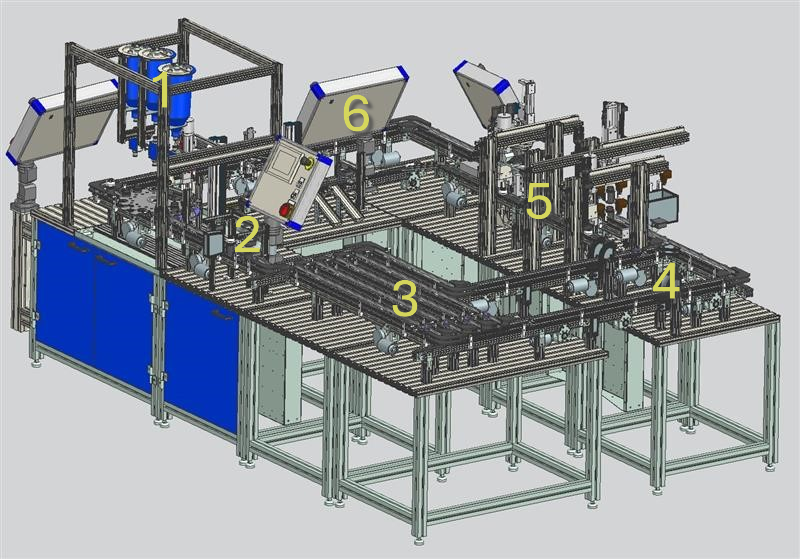
\includegraphics[width=0.8\textwidth]{figures/Bild.PNG}
    \caption{Stationen der SmartFactory-Anlage\cite{siemens2022}} 
    \label{fig:Stationen_SmartFactory} % Für spätere Verweise im Text.
    \vspace{0.5em} % Optional: Abstand zwischen Bildunterschrift und Zusatztext
    \small % Schriftgröße anpassen, falls gewünscht
\end{figure}

Abbildung 4.1 zeigt ein Modellbild der gesamten Anlage und veranschaulicht die räumliche Anordnung sowie die Verknüpfung der einzelnen Stationen. 
In den folgenden Abschnitten werden die Funktionsweisen der jeweiligen Module detailliert beschrieben.

\section{Station 1: Abfüllung (AS)}\label{sec:Station 2: Abfüllung}

Die Abfüllstation ist der Start des Kreislaufs der Anlage und hat die Aufgabe, Flaschen mit einer vorgegebenen Anzahl von Kugeln zu befüllen. 
Diese Anzahl wird durch 
die Erstellung von Aufträgen am Bedienpanel (HMI) oder Remote über Open Platform Communications Unified Architecture (OPC UA) auf einem 
Webinterface festgelegt. Hier kann zum Beispiel der Prozentsatz der Kugelfarbe (bei einem Maximum 
von 250 Kugeln) oder ein Absolutwert für die Anzahl der Kugeln festgelegt werden. Für das Abfüllen, hat die Abfüllung drei 
Container mit jeweils, roten, blauen und gelben Kugeln. Außerdem kann die Anzahl der abzufüllenden Flaschen angegeben 
werden. Diese Anzahl wird per ``On-Demand''-TCP-Verbindung an das Modulare Produktionssystem gesendet. Die danach von dem 
modulare Produktionssystem gesendeten Flaschen werden durch einen Drehteller an verschiedenen Verarbeitungsstationen bewegt. 
Als erstes wird die Flasche, mit der des Auftrages angegebenen Anzahl an Kugeln, an der ersten Verarbeitungsstationen befüllt 
(\ref{fig:Abfüllung}). Dann wird in Verarbeitungsstationen 2 (\ref{fig:Abfüllung}) ein Deckel von dem modulare 
Produktionssystem angefordert und von diesem auf die Flasche gesetzt. Der Deckel wird danach in Verarbeitungsstationen 3 
(\ref{fig:Abfüllung}) mit einen drehbaren Greifer verschraubt 
und an der vierten Verarbeitungsstationen (\ref{fig:Abfüllung}) wird der RFID-Tag im Deckel beschrieben. Der RFID-Tag enthält Datum und Uhrzeit der Abfüllung, sowie welcher 
Auftrag abgefüllt wurde. Jeder dieser Schritte wird parallel ausgeführt werden, um die Produktionszeit zu minimieren.

\begin{figure}[h!]
    \centering
    \includegraphics*{figures/Abfüllstation.png}
    \caption{Abfüllstation\cite{siemens2022}} % "Abbildung 2" wird automatisch eingefügt.
    \label{fig:Abfüllung} % Für spätere Verweise im Text.
\end{figure}
\FloatBarrier
\section{Station 2: Quality Gate (QG)}\label{sec:Station 3: Quality Gate}

Das Quality Gate gleicht die Auftragsdaten auf dem RFID-Tag mit dem Inhalt der Flasche ab. Hierzu wird an der ersten Verarbeitungsstation der 
RFID-Tag der Flasche eingelesen, und an der zweiten Verarbeitungsstation prüft ein Farbsensor die farbliche Zusammensetzung. Stimmt die farbliche 
Zusammensetzung überein, wird an der dritten Verarbeitungsstation der RFID-Tag der Flasche mit „Gut“ beschrieben. Stimmt sie nicht überein, 
wird der RFID-Tag mit „Ausschuss“ beschrieben. Jede Verarbeitungsstation hat dafür einen eigenen Vereinzelner, um die richtige Verarbeitung der 
Flaschen zu gewährleisten. Der Anlagenteil dient zur Qualitätssicherung der abgefüllten Flaschen.

\begin{figure}[h!]
    \centering
    \includegraphics*{figures/qualitygate.png}
    \caption{Quality Gate\cite{siemens2022}} % "Abbildung 2" wird automatisch eingefügt.
    \label{fig:QualityGate} % Für spätere Verweise im Text.
\end{figure}
\FloatBarrier
\section{Station 3: Kommissionierbahnen (KB)}\label{sec:Station 4: Kommissionierbahnen}

Die Kommissionierbahnen sortieren die vom Quality-Gate ankommenden Flaschen nach Auftragsnummer, hierzu wird zu Beginn der RFID-Tag gelesen und 
die Flasche auf eine von vier Bahnen sortiert. Durch das Quality-Gate als fehlerhaft markierte Flaschen oder Flaschen ohne lesbaren RFID-Chip 
werden direkt über ein Ausschussband an die nächste Station weitergegeben. Ist die Flasche “In Ordnung”, wird sie auf eine von vier Bändern 
sortiert. Die sortierten Flaschen bleiben in der Station, bis der entsprechende Auftrag abgeschlossen wurde oder der Bediener ein manuelles 
Entleeren der Bänder anfordert.

\begin{figure}[h!]
    \centering
    \includegraphics*{figures/Kommisonierbahn.png}
    \caption{Kommissionierbahnen\cite{siemens2022}} % "Abbildung 2" wird automatisch eingefügt.
    \label{fig:Kommissionierbahnen} % Für spätere Verweise im Text.
\end{figure}
\FloatBarrier
\section{Station 4: Eckstation (ES)}\label{sec:Station 5: Eckstation}

Die Eckstation dient als Übergangspunkt, an dem die Flaschen von der Kommissionierbahn zur Recyclingstation weitergeleitet werden.
Die Besonderheit der Eckstation sind, zwei Laufbänder, welche als hochklappbare Brücken fungieren, eine für die Abhandlung von 
Aufträgen und eine für aussortierte Flaschen. Das Hochklappen ermöglicht es, 
einen Schaltschrank in der Mitte der Anlage zu erreichen. Das Hochklappen der Laufbänder wird unterbunden, wenn 
noch Flaschen auf dem Laufband sind. Dies erfordert das Tracken der Flaschenanzahl und einen Stopper, um den Zulauf der 
Flaschen bei hochgeklappten Laufbändern zu verhindern und das Hochklappen bei vollem Laufband zu verhindern. Ist das 
Laufband voll, wird der Zulauf durch den Stopper verhindert. Des Weiteren ist es möglich, ein entsprechendes Anforderungssignal an die Eckstation,
zum Anheben der Brücke, zu senden, auf dessen Quittierung Flaschen warten müssen.
Die Station übernimmt keine weiteren Funktionen und dient ausschließlich dazu, die Flaschen zwischen den beiden Stationen zu verfahren und Zugang 
zum Einschaltschrank zu gewährleisten.

\begin{figure}[h!]
    \centering
    \includegraphics*{figures/eckstation.png}
    \caption{Eckstation\cite{siemens2022}} % "Abbildung 2" wird automatisch eingefügt.
    \label{fig:Eckstation} % Für spätere Verweise im Text.
\end{figure}
\FloatBarrier

Abbildung 4.5 zeigt den Aufbau der Eckstation. Die Kontaktpunkte für die versenkbaren Brücken befinden sich an den Sensoren BG4, BG5, BG11 und BG12. 
Diese Sensoren detektieren, ob die Brücken richtig in die ursprüngliche Position verfahren wurden.

\section{Station 5: Recycling (Recy)}\label{sec:Station 6: Recycling}

Die Recyclingstation übernimmt eine entscheidende Rolle im geschlossenen Produktionskreislauf der SmartFactory-Anlage. Sie verarbeitet alle 
ankommenden Flaschen, unabhängig davon, ob diese aus erfolgreich abgeschlossenen Produktionsaufträgen stammen oder aufgrund von Fehlern 
aussortiert wurden.

Zu Beginn wird jede Flasche von einem \textbf{RFID-Reader} erfasst, der ihre Identität und den Zustand überprüft. Diese Informationen werden an 
die Steuerung weitergeleitet, um den weiteren Verarbeitungsprozess zu optimieren. Anschließend gelangt die Flasche zum \textbf{Deckelentferner}, 
wo ein präziser Greifer den Flaschendeckel entfernt. Der Deckel wird auf ein separates Laufband transportiert, das die Deckel für eine spätere 
Verarbeitung zur Verfügung stellt (\ref{fig:Recycling}).

Nach der Entfernung des Deckels fährt die Flasche weiter zum \textbf{Entleerer}. Hier wird sie von einem Greifer angehoben und über einen 
Trichter positioniert, wo die Kugeln entleert werden (\ref{fig:Recycling}). Der Trichter ist mit einem 
\textbf{Farbsensor} ausgestattet, der die Farbe der Kugeln erkennt. Diese Information wird an das Steuerungssystem weitergegeben, um die 
Kugeln entsprechend zu sortieren.

Das Rückführungssystem für die Kugeln wird \textbf{pneumatisch} betrieben. Je nach erkannter Farbe wird der passende Abfüllschlauch 
aktiviert, durch den die Kugeln in den entsprechenden Container an der Abfüllstation geschossen werden. Dies gewährleistet eine exakte 
farbliche Trennung und ermöglicht die Wiederverwendung der Kugeln im weiteren Produktionszyklus.

Während die erste Flasche entleert wird, bereitet das System die nächste Flasche für den Deckelentfernungsprozess vor, um eine hohe Effizienz 
sicherzustellen. Nach dem Entleeren wird die Flasche wieder auf das Laufband gesetzt und zum \textbf{Modularen Produktionssystem (MPS)} 
weitergeleitet. Die MPS macht die Flasche anschließend für weitere Produktionszyklen verfügbar.

\begin{figure}[h!]
    \centering
    \includegraphics*{figures/recyclingstation.png}
    \caption{Recyclingstation\cite{siemens2022}} % "Abbildung 2" wird automatisch eingefügt.
    \label{fig:Recycling} % Für spätere Verweise im Text.
\end{figure}
\FloatBarrier

\section{Station 6: Modulares Produktionssystem (MPS)}\label{sec:Station 6: Modulares Produktionssystem}

Das Modulare Produktionssystem (MPS) ist eine zentrale Komponente der SmartFactory-Anlage und dient der Bereitstellung von Flaschen und 
Deckeln für die Abfüllstation. Es nimmt Deckel von der Recycling-Anlage entgegen, überprüft diese mithilfe eines RFID-Lesegeräts und 
eines Farbsensors auf Lesbarkeit und Farbe und sortiert fehlerhafte oder andersfarbige Deckel, wie rote, aus.

Auf Anforderung der Abfüllstation liefert das MPS die benötigte Anzahl an Flaschen und setzt mithilfe eines Greifers die passenden weißen 
Deckel auf die befüllten Flaschen. Fehlerhafte Flaschen oder Deckel werden aussortiert, um die Produktionsqualität zu sichern. Das System 
überwacht kontinuierlich den Materialvorrat, um Unterbrechungen zu vermeiden, und stellt relevante Daten über ein HMI bereit. 

\begin{figure}[h!] % "h!" zwingt die Position der Abbildung genau hier
    \centering
    \includegraphics*{figures/mps.png}
    \caption{Modulares Produktionssystem\cite{siemens2022}} % "Abbildung 2" wird automatisch eingefügt.
    \label{fig:MPS} % Für spätere Verweise im Text.
\end{figure}
\FloatBarrier

\section{Netzwerkverbund}\label{sec:Netzwerkverbund}

Alle Anlagenteile sind via Ethernet mit der Einspeisung verbunden und bilden damit ein Subnetz. Dies ermöglicht eine 
effiziente und stabile Kommunikation zwischen den verschiedenen Stationen der Anlage und ermöglicht das Senden und Empfangen von Daten.
Die gesamte Kommunikation der Anlage erfolgte “On-Demand” und passiert dadurch nur wenn sie von einer anderen Station angefordert wird.

\section{Begriffsklärungen}\label{sec:Begriffsklärungen}

\textbf{Totally Integrated Automation (TIA):}

Im nachfolgenden Abschnitt wird das programmieren von speicherprogrammierbaren Steuerungen (SPS) mit hilfe von Totally Integrated Automation (TIA) 
mehrfach thematisiert. Dabei handelt es sich um die Entwicklungsumgebung für alle Automatisierungsprodukte von Siemens \cite{bee2022}.

Eine speicherprogrammierbare Steuerung (SPS) ist ein digitales Gerät, das zur Steuerung von Maschinen und Anlagen eingesetzt wird.
Die Prozesslogik für speicherprogrammierbare Steuerung (SPS) lässt sich in verschiedenen Programmiersprachen umsetzen, 
darunter FUP (Funktionsplan), AWL (Anweisungsliste) und SCL (Structured Control Language). Für die SmartFactory-Anlage 
wurde festgelegt, die Programmierung bedarfsgerecht in FUP und SCL durchzuführen.

Da eine speicherprogrammierbare Steuerung (SPS) als Echtzeitsystem zyklisch arbeitet, sie führt 
Berechnungen durch und aktualisiert Ausgaben in Intervallen, sind bei der Programmierung spezielle Anforderungen 
zu beachten. Dafür stehen verschiedene Konzepte zur Verfügung:

\begin{itemize}
    \item \textbf{Funktion:} Ähnlich wie eine Methode in C\#, ermöglicht eine Funktion die Verarbeitung von Übergabeparametern 
    und die Berechnung entsprechender Ausgabewerte. Allerdings sind diese Ausgabewerte nicht persistent, da sie in jedem 
    Programmzyklus neu berechnet werden.
    \item \textbf{Funktionsbaustein:} Ein Funktionsbaustein bietet dieselben Möglichkeiten wie eine Funktion, jedoch mit der 
    zusätzlichen Fähigkeit, Daten über mehrere Zyklen hinweg zu speichern.
    \item \textbf{Datenbaustein:} Ein Datenbaustein dient der persistenten Speicherung von für das Programm relevanten Daten. 
    Wird ein Funktionsbaustein erstellt, wird automatisch ein zugehöriger Datenbaustein zur Speicherung seiner Daten angelegt.
    \item \textbf{User Defined Datatype (UDT):} Ein UDT ist ein benutzerdefinierter Datentyp, der individuell vom 
    Programmierer erstellt werden kann. Er ermöglicht die Zusammenfassung mehrerer Variablen in einem einzigen Datentyp und 
    wird vorallem für die Softwarekonfiguration einselnder Module verwendet.
\end{itemize}

\textbf{Konzeptionierung nach ISA-88:}

Die Software der Anlage wurde gemäß dem ISA-88-Standard konzipiert. Dieser Standard legt fest, dass die Software in 
wiederverwendbare Module für Bauteile und Baugruppen strukturiert wird. Die Module wurden in die folgenden Typen unterteilt:

\sloppy
\begin{itemize}
    \item \textbf{Control Modul:} Ein Control Modul repräsentiert einzelne Bauteile, die an jeder Station der Anlage
    vorkommen. Ein typisches Beispiel ist ein Sensor. Obwohl an der Anlage verschiedene Sensortypen verbaut sind, teilen 
    sie alle die grundlegende Funktion, ein Bit umzuschalten. Das Control Modul \texttt{CM\_BinarySensor} ist so entwickelt 
    worden, dass es universell für alle Sensortypen von Siemens einsetzbar ist, wobei lediglich die Hardwareadresse des jeweiligen 
    Sensors angegeben werden muss.

    \item \textbf{Equipment Modul:} Equipment Module bestehen aus einer Kombination mehrerer, aber mindestens einem Control Module\footnote{Vgl. ResearchGate, \url{https://www.researchgate.net/figure/SA-88s-physical-model-and-an-example-production-allocation_fig2_308384237/}, zuletzt aufgerufen am 11. Januar 2025.}
    und bilden komplexere Baugruppen ab. Beispielsweise sind an den Förderbändern der SmartFactory-Anlage neben Sensoren auch 
    Pneumatikzylinder verbaut. Da die Anzahl der Control Module pro Förderband variieren kann, wurde das Equipment Modul 
    \texttt{EM\_Conveyor} so gestaltet, dass es eine beliebige Anzahl an Control Modulen unterstützt und flexibel 
    konfigurierbar ist.

    \item \textbf{Unit:} Die Unit bildet die spezifische Prozesslogik eines Anlagenmoduls ab und implementiert die 
    erforderlichen Programmabläufe.
\end{itemize}

Die Struktur eines nach ISA-88 entworfenen Systems ist hierarchisch organisiert. In diesem Aufbau kommuniziert eine Unit 
ausschließlich mit Equipment Modulen, während Equipment Module sowohl mit Units als auch mit Control Modulen interagieren. 
Control Module hingegen stehen nur in Verbindung mit Equipment Modulen.
